\section[VAN]{VAN}
	\begin{equation}
	\label{eq:van}
	\begin{split}
 		w = - C_0 + \sum_{k=1}^n \frac{CF_k}{(1+r)^k}
	\end{split}
	\end{equation}
	Consideriamo, quindi, il valore del \ac{VAN} su $12$ flussi di cassa (\textit{cashflow}), corrispondenti alle stime sull'utile realizzato alla fine di ogni mese ed un \textbf{tasso di sconto} $r$ pari al \textbf{\ac{WACC}} (\ref{eq:wacc_tax_value}).\newline
	La formula (\ref{eq:van}) diventa, quindi:	
	\begin{equation}
	\label{eq:van_caso_studio}
	\begin{split}
 		w = - C_0 + \sum_{k=1}^{12} \frac{CF_k}{(1+0,01726)^k}
	\end{split}
	\end{equation}	
	Il valore $C_0$ corrisponde all'investimento iniziale del nostro progetto, quindi, pari al \textbf{CAPEX} $ 56\thinspace 170,20 \: \mbox{\euro}$.
	Assumiamo, inoltre, che i flussi mensili siano costanti nell'arco di un anno, quindi la quantità $CF_k$ non è più legata al k-esimo mese ma si può esprimere come $CF$ pari a:
	\begin{equation}
	\label{eq:flussi_cassa_mensili}
	\begin{split}
 		CF = x \:(fatturato \: mensile) - 60\thinspace 131,27 \: (OPEX)
	\end{split}
	\end{equation}	  	
la (\ref{eq:van_caso_studio}) diventa (il VAN diventa funzione dei flussi di cassa lordi $x$ quindi $w = y(x)$):	
	\begin{eqnarray}
	\label{eq:van_caso_studio_2}
 		y(x) & = & - 56\thinspace 170,20 + \sum_{k=1}^{12} \frac{x - 60\thinspace 131,27}{(1+0,01726)^k} \nonumber \\
 		 & = & -56\thinspace 170,20 + (x - 60\thinspace 131,27) \cdot \underbrace{\sum_{k=1}^{12} \frac{1} {(1+0,01726)^{k}}}_{{}=10,7528} \nonumber \\
 		 & = & -56\thinspace 170,20 + (x - 60\thinspace 131,27) \cdot 10,7528 \nonumber \\
 		 & = & -702\thinspace 749,72 + 10,7528 \cdot x 		
	\end{eqnarray}  		

	\begin{comment}	
	ci possiamo, quindi, calcolare il valore del \ac{TIR} corrispondente. Per definizione il \ac{TIR} è pari a:
	\begin{equation}
	\label{eq:tir}
	\begin{split}
 		\sum_{k=0}^n \frac{C_k}{(1+i)^k} = 0
	\end{split}
	\end{equation}	 

	\end{comment}
 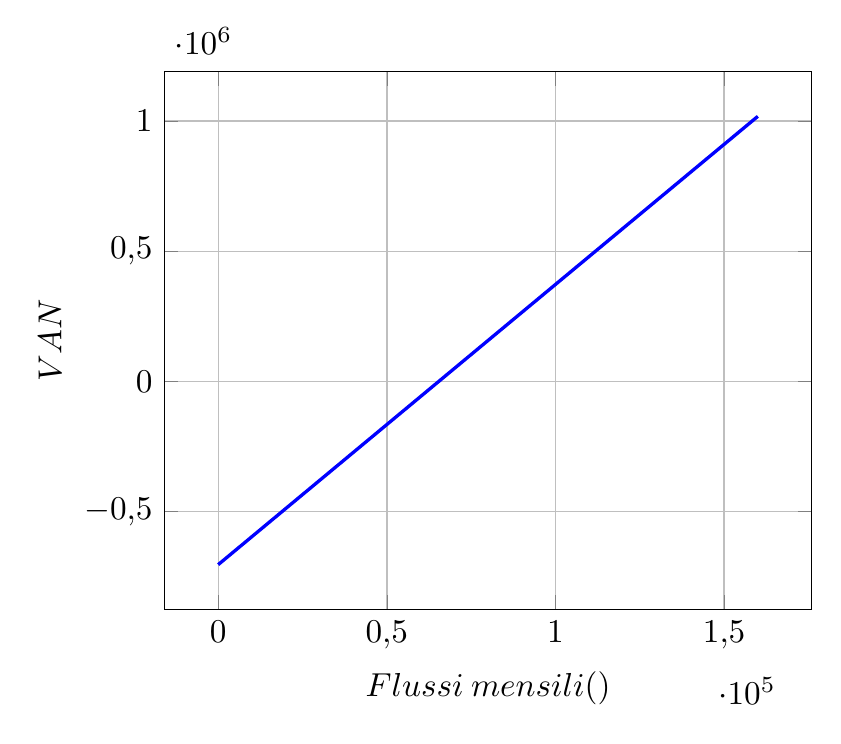
\begin{tikzpicture}[scale=1.2]
 \pgfkeys {
			/pgf/number format/.cd,
			set decimal separator={,{\!}},
			set thousands separator={}}
	\begin{axis}[ xlabel=$Flussi\: mensili (\mbox{\euro})$, 
				   ylabel=$VAN$, 
				   grid=major ]
		
		\addplot[domain=0:160000, color=blue, line width=1pt]{10.7528 * x - 702749.72};
		
	\end{axis}
\end{tikzpicture}

Un punto importante della funzione (\ref{eq:van_caso_studio_2}) è quello per cui il $ VAN = 0 $, ovvero:

	\begin{equation}
	\label{eq:van_zero}
	\begin{split}
 		y(x) = 0
 	\end{split}
	\end{equation}

Il valore $x$ per cui (\ref{eq:van_zero}) è soddisfatta 
	\begin{equation}
	\label{eq:van_pareggio_1}
	\begin{split}
 		10,7528 \cdot x - 702\thinspace 749,72 = 0	
 	\end{split}
	\end{equation}
è pari a:
	\begin{eqnarray}
	\label{eq:van_pareggio_2}
		x & = & \frac{702\thinspace 749,72	}{10,7528}	 	\nonumber \\[1.5ex] 
		  & = &  65\thinspace 355,04 \: \mbox{\euro} 
	\end{eqnarray}
Il valore di $x$ rappresenta, da un punto di vista fisico, il flusso minimo di cassa che dovremmo registrare per avere il progetto remunerativo. Infatti, se per i prossimi 12 mesi registrassimo un flusso di cassa pari a (\ref{eq:van_pareggio_2}) riusciamo a recuperare il 31 Dicembre la somma investita il 1 Gennaio per avviare la nostra azienda, per definizione di VAN:
%
%	Tabella relativa alla valutazione VAN = 0,00
%
\begin{savenotes}
\begin{table}[htb]
\centering
 \caption{VAN}
 \begin{tabular}{D{,}{,}{3.2}D{,}{,}{7.2}D{,}{,}{7.2}}
 \toprule
 	\multicolumn{1}{c}{\textbf{Mese}} & \multicolumn{1}{c}{\textbf{Flussi di cassa netti (\euro)}} & \multicolumn{1}{c}{\textbf{Flussi di cassa attualizzati (\euro)}} \\
 \midrule	
 	1 & 5\thinspace 223,80 & 5\thinspace 134,97 \\ 
 	2 & 5\thinspace 223,80 & 5\thinspace 047,67 \\
 	3 & 5\thinspace 223,80 & 4\thinspace 961,80 \\ 
 	4 & 5\thinspace 223,80 & 4\thinspace 877,42 \\
 	5 & 5\thinspace 223,80 & 4\thinspace 794,48 \\ 
 	6 & 5\thinspace 223,80 & 4\thinspace 712,94 \\
 	7 & 5\thinspace 223,80 & 4\thinspace 632,80 \\ 
 	8 & 5\thinspace 223,80 & 4\thinspace 554,01 \\
 	9 & 5\thinspace 223,80 & 4\thinspace 476,57 \\ 
 	10 & 5\thinspace 223,80 & 4\thinspace 400,44 \\
 	11 & 5\thinspace 223,80 & 4\thinspace 325,61 \\ 
 	12 & 5\thinspace 223,80 & 4\thinspace 252,05 \\ 	
	\midrule
	 & \textbf{TOTALE (\euro)} & 56\thinspace 170,72 \\		
 \bottomrule
 \end{tabular} 
 \label{table:van_zero}
\end{table}
\end{savenotes}
Da un punto di vista grafico si osserva come il punto di coordinate \textbf{\textcolor{blue}{( 65355,04 ; 0 )}} rappresenti il \textit{punto di frontiera} tra due aree che presentano delle caratteristiche diverse, quella:
\begin{itemize}
\item \textbf{\color{red}{rossa}} è caratterizzata da tutti i flussi di cassa che \underline{non} permettono di rientrare dell'investimento ( pertanto il VAN è negativo );
\item \textbf{\color{green}{verde}} da tutti quei flussi per cui è possibile recuperare i CAPEX sostenuti all'avvio della società. Ovviamente maggiore saranno i flussi più breve risulterà il \textbf{periodo di pareggio}.
\end{itemize}

\usepgfplotslibrary{fillbetween}

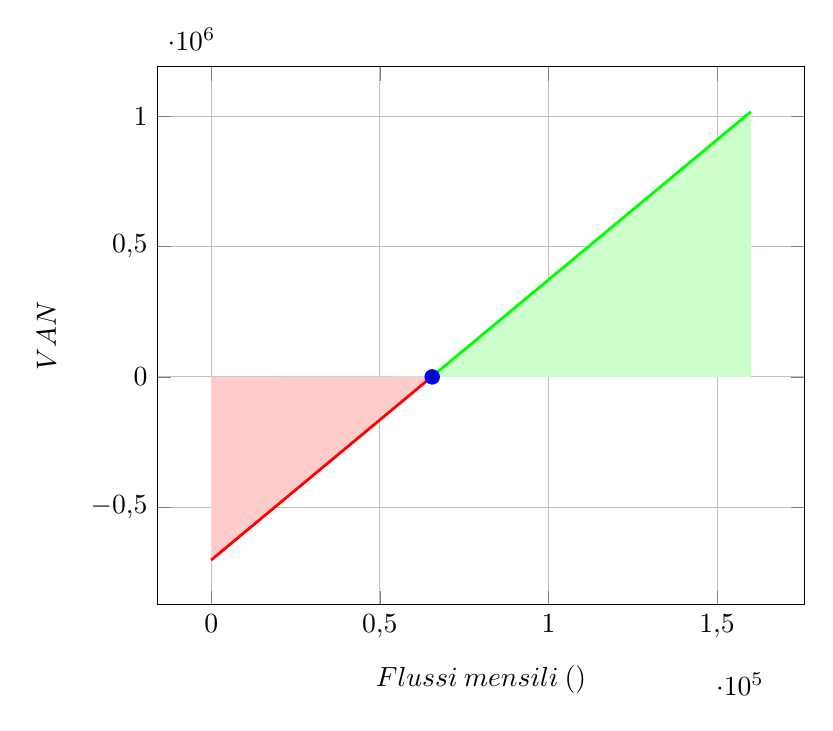
\begin{tikzpicture}[scale=1.2]
 \pgfkeys {
			/pgf/number format/.cd,
			set decimal separator={,{\!}},
			set thousands separator={}}

    \begin{axis}[thick,smooth, xlabel=$Flussi \: mensili \:(\mbox{\euro})$, ylabel=$VAN$, grid=major]    

		\addplot coordinates{( 65535, 0) };
							  
        \addplot+[domain=0:65535, name path=A,red,line width=1pt, no markers] {10.7528 * x - 702749.72};
        \addplot+[domain=65535:160000, name path=C,green,line width=1pt, no markers] {10.7528 * x - 702749.72};
        \addplot+[domain=0:160000, name path=B, draw=none,black, no markers] {0};

        \addplot[domain=0:65535, red!20] fill between[of=A and B];
        \addplot[domain=65535:160000, green!20] fill between[of=C and B];
    \end{axis}
\end{tikzpicture}


\begin{comment}
\subsection[Break-even period]{Break-even period}
	Si analizza, infine, il \textbf{punto di pareggio}, ovvero la quantità di chiamate necessarie per avere un fatturato tale da ricoprire l'investimento iniziale, in modo tale da chiudere il periodo di riferimento senza perdite né profitti.

Il \textbf{break even period} (periodo di pareggio), ovvero il periodo di tempo necessario per il recupero dell'esborso iniziale è quindi pari a:   	
\end{comment}
%
%	Tabella relativa al caso teorico in cui non ci siano malati durante un anno
%
\begin{savenotes}
\begin{table}[htb]
\centering
 \caption{Variazione VAN (Caso Teorico)}
 \begin{tabular}{p{4cm}D{,}{,}{5.2}D{,}{,}{5.2}D{,}{,}{5.2}D{,}{,}{7.4}}
 \toprule
 	& \multicolumn{1}{c}{Flusso di cassa mensile (\euro)} & \multicolumn{1}{c}{Contratti Mensili } &\multicolumn{1}{c}{\textbf{VAN}}&\multicolumn{1}{c}{\textbf{ \% Contratti}} \\
 \midrule	
	\makebox[4cm][r]{Ottimo} & 553\thinspace 419,36 & 8\thinspace 138,52 & 5\thinspace 248\thinspace 057,65 & 1,0000\\
 	\makebox[4cm][r]{Pareggio} & 65\thinspace 355,07 & 939,18 & 0,00 & 0,1154\\ 
 \bottomrule
 \end{tabular} 
\end{table}
\end{savenotes}